\chapter{Assignment \#7: Fuel Pin Thermal Analysis}
\label{ch:ass7}


\begin{fullwidth}
\newthought{Consider a} fuel pin with the following parameters:
\begin{table}
\begin{tabular}{l | l}
\toprule
Temperature on outer surface of fuel pin & 630$^{\circ}$C \\
\hline
Linear heat rate & 33.0 kW/m \\
\hline
Fuel density & 95\% of theoretical density \\
\hline
Gadolinium weight fraction & 5\% \\
\hline
Burnup & 25 GWD/MT$_{\text{ihm}}$ \\
\bottomrule
\end{tabular}
\end{table}

\begin{figure}
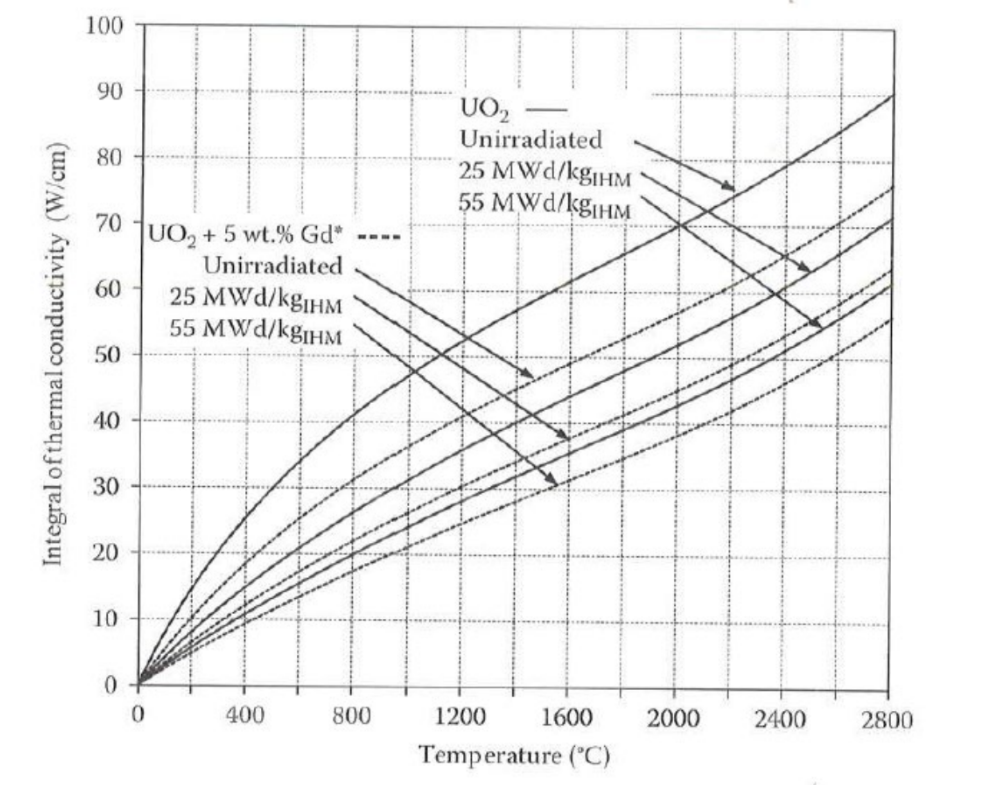
\includegraphics[width=10.0cm]{integral_of_fuel_thermal_conductivity.png}
\caption{Integral of fuel thermal conductivity.}
\label{fig:integral-of-fuel-thermal-conductivity}
\end{figure}
\begin{enumerate}
\item Use Figure \ref{fig:integral-of-fuel-thermal-conductivity} to estimate the fuel centerine temperature ($^{\circ}$C) under the given conditions.

\vspace{1.0 cm}

\item Implement the FRAPCON model in MATLAB to compute the fuel centerline temperature.

\vspace{1.0 cm}

\item With your MATLAB implementation of the FRAPCON model, estimate fuel centerline temperature for 97\% and 92\% theoretical density.

\vspace{1.0 cm}

\item Repeat your analysis using the FRAPCON model for the conditions given in the table above but with Gadolinium weight fraction changed to 0\% and begining of life. (Burnup = 0)

\vspace{1.0 cm}

\item Repeat the calculation of the previous problem but use the AREVA fuel thermal conductivity model (which you should implement in MATLAB) which gives thermal conductivity in units of W/m-K for UO$_2$ fuel at full theoretical density. 

The AREVA model is as follows:
\begin{align*}
k_{\text{TD}} &= \frac{1}{A_1 + A_2 T + A_3 \text{BU} + A_4 f(T)} + g(T) \\
A_1 &= 0.0375 \text{ m-K/W} \\
A_2 &= 2.165 \times 10^{-4} \text { m/W} \\
A_3 &= 1.70\times 10^{-3} \text{ m-K/W/(GWd/MT}_{\text{IHM}}\text{)} \\
A_4 &= 0.058 \text{ m-K/W} \\
f(T) &= \left[1 + \exp{\left(\frac{T-900}{80} \right)} \right]^{-1} \\
g(T) &= 4.715 \times 10^{9} T^{-2} \exp{\left(-\frac{16,361}{T} \right)} \text{ W/m-K} \\
\end{align*}
\end{enumerate}


\end{fullwidth}
